% Asset ID: AS2CorrelationAndRegressionLinesTikZ-004
% Source: CCEA AS2-DPI-LO006 + S1-Chp4-Correlation.pdf page 12 + transcript
% Related section: Core Theory - Interpolation and extrapolation
% Purpose: Show interpolation inside the observed range and extrapolation outside it.
\documentclass[tikz,border=6pt]{standalone}
\usepackage{amsmath}
\usetikzlibrary{arrows.meta,patterns}
\begin{document}
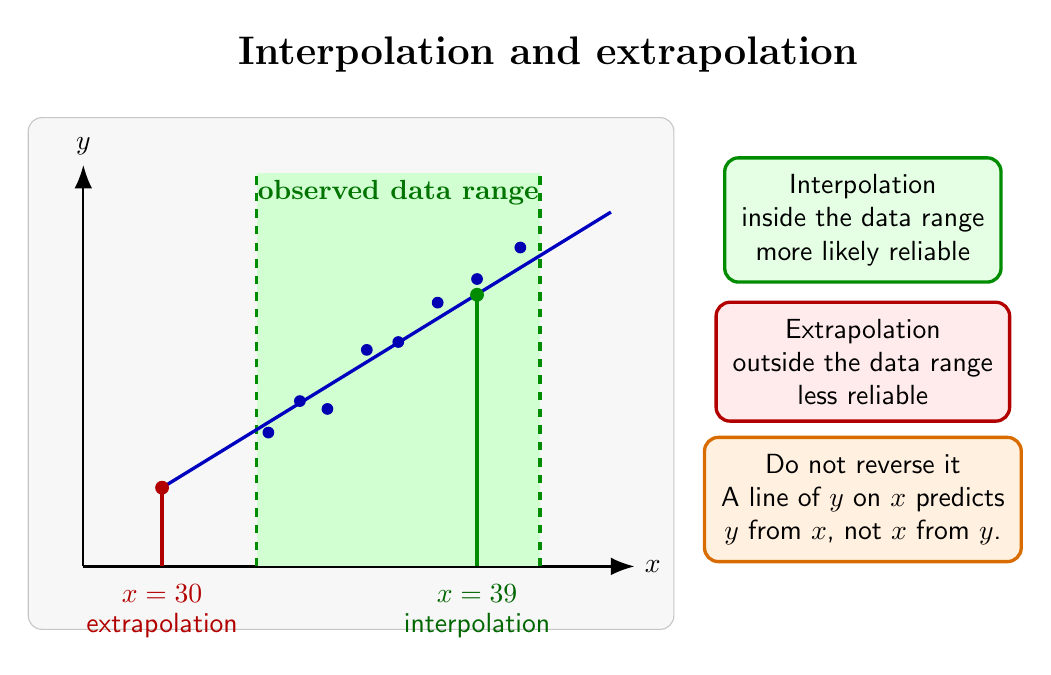
\begin{tikzpicture}[font=\sffamily,>={Latex[length=3mm]},point/.style={circle, fill=blue!70!black, inner sep=1.5pt},card/.style={draw, rounded corners=5pt, very thick, align=center, inner sep=6pt}]
\node[font=\bfseries\Large] at (5.9,6.5) {Interpolation and extrapolation};
\draw[rounded corners=5pt, fill=gray!6, draw=gray!45] (-0.7,-0.8) rectangle (7.5,5.7);
\draw[->, thick] (0,0) -- (7,0) node[right] {$x$};\draw[->, thick] (0,0) -- (0,5.1) node[above] {$y$};
\fill[green!18] (2.2,0) rectangle (5.8,5.0);\draw[green!55!black, very thick, dashed] (2.2,0) -- (2.2,5.0);\draw[green!55!black, very thick, dashed] (5.8,0) -- (5.8,5.0);\node[green!45!black, font=\bfseries] at (4,4.75) {observed data range};
\draw[very thick, blue!75!black] (1.0,1.0) -- (6.7,4.5);\foreach \p in {(2.35,1.7),(2.75,2.1),(3.1,2.0),(3.6,2.75),(4.0,2.85),(4.5,3.35),(5.0,3.65),(5.55,4.05)}\node[point] at \p {};
\draw[very thick, green!55!black] (5.0,0) -- (5.0,3.45);\fill[green!55!black] (5.0,3.45) circle (2.5pt);\node[green!40!black, font=\bfseries] at (5.0,-0.35) {$x=39$};\node[green!40!black] at (5.0,-0.75) {interpolation};
\draw[very thick, red!70!black] (1.0,0) -- (1.0,1.0);\fill[red!70!black] (1.0,1.0) circle (2.5pt);\node[red!70!black, font=\bfseries] at (1.0,-0.35) {$x=30$};\node[red!70!black] at (1.0,-0.75) {extrapolation};
\node[card, fill=green!10, draw=green!55!black] at (9.9,4.4) {Interpolation\\inside the data range\\more likely reliable};\node[card, fill=red!8, draw=red!70!black] at (9.9,2.6) {Extrapolation\\outside the data range\\less reliable};\node[card, fill=orange!12, draw=orange!85!black] at (9.9,0.85) {Do not reverse it\\A line of $y$ on $x$ predicts\\$y$ from $x$, not $x$ from $y$.};
\end{tikzpicture}\end{document}
